\chapter{História Estatística}

A maior parte da visualização de dados é feita para fins de comunicação. Temos uma visão sobre um conjunto de dados, temos um público potencial e gostaríamos de transmitir nossa visão ao nosso público. Para comunicar nossa visão com sucesso, teremos que apresentar ao público uma história clara e emocionante. \vskip0.3cm

A necessidade de uma história pode parecer perturbadora para cientistas, jornalistas e Agentes Públicos, que podem equipará-la a inventar coisas, dar uma guinada nas coisas ou exagerar nos resultados. No entanto, essa perspectiva perde o importante papel que as histórias desempenham no raciocínio e na memória.\vskip0.3cm

Os cientistas frequentemente sabem como visualizar dados sem serem grosseiramente enganosos. No entanto, eles podem não ter um senso de estética visual bem desenvolvido e podem, inadvertidamente, fazer escolhas visuais que prejudicam a mensagem desejada. Os designers, por outro lado, podem preparar visualizações que parecem bonitas, mas jogam rápido e solto com os dados. 

%(WILKE, 2019). 
\section{O Que é uma História Estatística}

Por conta própria, as estatísticas são apenas números. Eles estão em toda parte em nossa vida. Os números aparecem em histórias esportivas, relatórios sobre a economia, atualizações do mercado de ações, para citar apenas alguns. Para significar alguma coisa, seu valor para a pessoa na rua deve ser trazido à vida.\vskip0.3cm 

Uma história é um conjunto de observações, fatos ou eventos, verdadeiros ou inventados, que são apresentados em uma ordem específica para criar uma reação emocional no público.\vskip0.3cm 

Uma história estatística é aquela que não apenas recita dados em palavras. Ele conta uma história sobre os dados. Os leitores tendem a se lembrar de ideias com mais facilidade do que dos dados. Já, uma história estatística transmite uma mensagem que conta aos leitores o que aconteceu, quem fez, quando e onde aconteceu e, esperançosamente, por que e como aconteceu.\vskip0.3cm 

Uma História Estatística pode:

\begin{itemize}
    \item Fornecer conhecimento geral, algumas perspectiva, e um certo contexto;
    \item Informar o debate sobre algumas questões específicas.
\end{itemize}


Em termos jornalísticos, o número por si só não é a história. Uma história estatística mostra aos leitores o significado, a importância e a relevância das informações mais atuais. Em outras palavras, responde à pergunta: por que meu público deveria querer ler sobre isso?\vskip0.3cm 

Finalmente, uma história estatística deve conter material digno de nota. Pergunte a si mesmo: a informação é suficientemente importante e inovadora para atrair a cobertura da mídia? A mídia pode escolher um foco diferente. Mas eles têm muitos outros fatores a considerar ao escolher um enredo.

Contar histórias estatísticas é sobre:

\begin{itemize}
    \item Chamar a atenção do leitor com um título ou imagem;
    \item Fornecer a história por trás dos números de forma fácil de entender, interessante e divertida;
    \item Encorajar leitores e outros a considerar como as estatísticas podem adicionar impacto a quase todas as histórias que eles têm para contar.
\end{itemize}

\section{Por Que Contar uma História Estatística}

Uma fonte estatística deve querer contar uma história sobre seus dados por pelo menos dois motivos.\vskip0.3cm 

Primeiro, o mandato da maioria das agências é informar o público em geral sobre a população, sociedade, economia e cultura da nação.\vskip0.3cm 

Essas informações orientarão os cidadãos na realização de seus trabalhos, na criação de suas famílias, nas compras e na tomada de muitas outras decisões.
Em segundo lugar, uma agência deve querer demonstrar a relevância de seus dados para o governo e o público.\vskip0.3cm 

Dessa forma, pode antecipar maior apoio público a seus programas, bem como melhorar o relacionamento com os entrevistados e maior visibilidade de seus produtos.\vskip0.3cm 

A maioria das agências conta principalmente com dois meios de comunicação de informações sobre as condições econômicas e sociais de um país e de seus cidadãos: a Internet e a mídia.\vskip0.3cm 

A Internet tornou-se uma ferramenta importante para facilitar o acesso às informações da agência. Mais e mais membros do público acessam os dados de uma agência diretamente em seu site. Ainda assim, a maioria dos cidadãos obtém suas informações estatísticas da mídia e, de fato, a mídia continua sendo o principal canal de comunicação entre os institutos de estatística e o público em geral.\vskip0.3cm 


Uma maneira eficaz de um escritório de estatística se comunicar por ambos os meios é contar uma história estatística escrita da forma mais clara, concisa e simples possível. O objetivo da Internet é informar melhor o público por meio do acesso direto. Ao escrever para a mídia, o objetivo é obter uma cobertura positiva, precisa e informativa.\vskip0.3cm 

As estatísticas podem dizer às pessoas algo sobre o mundo em que vivem. Mas nem todo mundo é adepto de entender as estatísticas por conta própria. Consequentemente, as histórias estatísticas podem e devem fornecer uma ajuda.
Por último, mas não menos importante, a disponibilidade de estatísticas depende, em primeiro lugar, da cooperação voluntária dos respondentes da pesquisa. As agências estatísticas não podem confiar apenas em sua autoridade legal para garantir uma taxa de resposta adequada.\vskip0.3cm 


A disponibilidade de estatísticas também depende de até que ponto os entrevistados entendem que os dados servem a um propósito importante ao fornecer um espelho do mundo em que vivemos. Quanto mais uma agência estatística puder mostrar a relevância de seus dados, mais os entrevistados serão encorajados a fornecer os dados.\vskip0.3cm 

 As histórias estatísticas e os dados que elas contêm devem ser informativos e iniciar a discussão, mas nunca devem estar abertos à discussão. Em outras palavras, as informações devem ser precisas e a integridade da Fonte nunca deve ser questionada. As histórias devem ser baseadas em dados de alta qualidade que sejam adequados para descrever os problemas que abordam.\vskip0.3cm 

 As Fontes devem sempre garantir a confidencialidade dos dados de pessoas físicas ou jurídicas. Na verdade, as histórias estatísticas não podem identificar ou revelar de forma alguma dados sobre indivíduos ou empresas.\vskip0.3cm 



 \section{Dados: Novo Petróleo do Mundo?}

Em 2006, o matemático e mepresário britânico e mentor de marketing da Tesco, \textbf{Clive Humby}, gritou dos telhados para o mundo: \textbf{Data Is The New Oil}. Em tradução livre para o significado original \textbf{“Os Dados São o Novo Petróleo”}, a frase que agitou o mundo dos negócios foi criada por um matemático especializado em ciência de dados. Desde 2014, ele é Cientista Chefe de Dados da empresa de insights do consumidor, \textbf{Starcount}. \vskip0.3cm 




“Os dados são o novo petróleo”, afirmou o então CEO da Mastercard, \textbf{Ajay Banga}, em um evento realizado em 2021, em São Paulo. O mantra passou a ser repetido por consultores, executivos e interessados em transformação digital. A fala e comparação faz sentido, exceto por um pequeno detalhe. “A diferença é que o petróleo vai acabar um dia”, ressaltou Banga.\vskip0.3cm 



Nos dias atuais, vivemos uma evolução foi muito grande e muito rápida, principalmente nos últimos 5 anos, na capacidade das empresas em coletar, processar, organizar e armazenar uma grande quantidade de dados dos seus clientes. Os dados viraram o novo petróleo do mmundo e combustível para o futuro.\vskip0.3cm 


%\begin{figure}[!htb]
%\centering
% 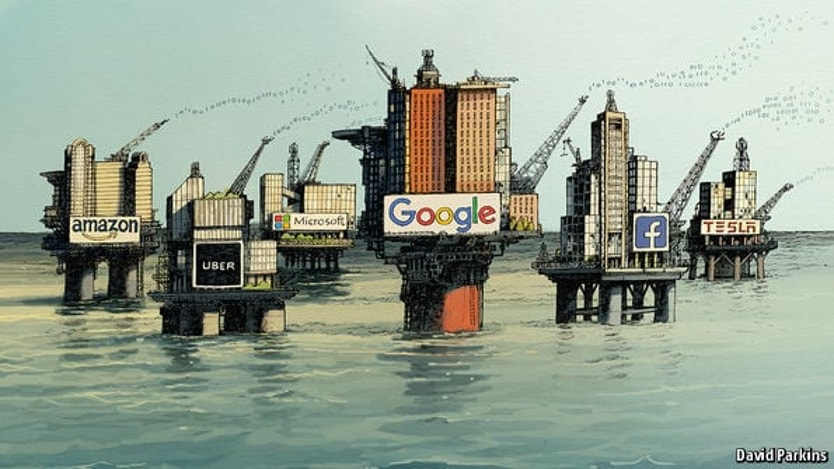
\includegraphics[scale=0.50]{figures/dados.jpg}\\
%  \vspace{-0.8cm}
%  \caption{O recurso mais valioso do mundo não é mais o petróleo, mas os dados}
%  \label{cantor1}
%\end{figure}





 Em 2017, \textbf{The Economist} publicou uma história intitulada: "O recurso mais valioso do mundo não é mais o petróleo, mas os dados". Desde a sua publicação, o tema gerou muita discussão, e "Dados são o novo petróleo" tornou-se um refrão comum . O problema é que a discussão geralmente se concentra em por que isso é uma coisa ruim.\vskip0.3cm 


Claro, existem preocupações legítimas sobre como os gigantes da tecnologia estão explorando o que sabem sobre nós. Mas, ao mesmo tempo, existem inúmeras maneiras pelas quais todos esses dados podem (e o fazem) melhorar o mundo. Vamos examinar alguns exemplos.\vskip0.3cm 


A \textbf{Harvard Medical School} publicou em 2016, uma pesquisa comparando a precisão dos sistemas de aprendizado de máquina contra patologistas humanos na detecção de câncer de mama. O aprendizado de máquina foi 92\% preciso, o que é bom. Mas os humanos foram 96\% precisos. Caso encerrado, certo?\vskip0.3cm 


Uma equipe de pesquisa da Harvard Medical School e do Beth Israel Deaconess Medical Center, desenvolveram métodos de inteligência artificial (IA) destinados a treinar computadores para interpretar imagens de patologia, com o objetivo de longo prazo de construir sistemas baseados em IA para tornar os diagnósticos patológicos mais precisos.\vskip0.3cm 



Harvard então combinou as descobertas dos patologistas com as varreduras dos sistemas de aprendizado de máquina. A precisão subiu para 99,5\%. Isso reduz os erros em quase uma ordem de magnitude (de 40 por mil para apenas 5 por mil) e representa 56.000 varreduras de mama mal interpretadas a menos por ano apenas nos EUA.\vskip0.3cm 

Os veículos autônomos (AVs) estão chegando. Os benefícios são amplamente conhecidos: estradas mais seguras, um impulso para a economia e menos aglomeração na hora do rush. Mas talvez o maior benefício seja a redução dos gases de efeito estufa (GEE) provenientes dos automóveis. Pesquisas conduzidas por professores da Universidade de Poznan estimam que os veículos autônomos podem eventualmente reduzir o GEE em 40\% a 60\%. Segundo a Agência de Proteção Ambiental, o transporte hoje responde por 29\% dos GEE nos Estados Unidos, então isso seria um avanço importante.\vskip0.3cm 

Como chegamos ao futuro AV? Você adivinhou: dados. Nesse caso, são necessárias centenas de petabytes de dados que formam o data lake do qual virão as soluções avançadas de aprendizado de máquina AV autônomo. Não para por aí. Cada uma dessas modernas "plataformas de computação que são móveis" gerará terabytes de dados por semana por veículo. Mesmo assumindo uma redução de 75\% no número de veículos nas estradas, são muitos exabytes de dados por ano.\vskip0.3cm 


 \subsection{Dados São Conhecimento e Isso Basta?}
 
 \textbf{Charliton Albert}, um político suíço que recebeu o Prêmio Nobel da Paz no início do século passado, falava que “Conhecimento é saber que um tomate é fruta. Sabedoria é saber que não se deve usar um tomate em uma salada de frutas.”\vskip0.3cm 

Creio que esta frase simboliza perfeitamente o cenário de dados que vivemos hoje em dia nas empresas, porque ter grande capacidade de captar, armazenar, analisar os dados e fazer campanhas de marketing, por exemplo, para mim, está no nível do conhecimento. E, sinceramente, esta é a parte mais fácil do trabalho exatamente porque hoje em dia temos acesso a ferramentas e tecnologias que auxiliam e potencializam este conhecer dos dados através de análises, modelos, machine learning e até inteligência virtual, mostrando tudo em dashboards de encher os olhos visualmente falando (porque às vezes os números que mostram enchem os olhos só de lágrimas). Só que isso está deslumbrando muitos profissionais e empresas.\vskip0.3cm 


\newpage
Os dados aqui são os nossos tomates, ou seja, temos muitos dados e conhecimento sobre eles, mas entendo que a maioria ainda está muito longe de transformar este conhecimento todo em sabedoria.\vskip0.3cm 

Então se os dados estão aí disponíveis para todos, o novo petróleo agora é ter a capacidade de analisar e usar estes dados com sabedoria, entendendo que nem sempre o que os dados dizem de maneira fria devem ser aplicados ou devem virar verdades absolutas. Em outras palavras, esta sabedoria fará a empresa não colocar os seus tomates em uma salada de frutas, mesmo que o banco de dados diga que tomate é uma fruta.\vskip0.3cm 

Para \textbf{César Ripari} diretor de Pré-Vendas da Qlik em uma entrevista em 2019, é seguro afirmar que a maior riqueza se encontra não nos dados em si, mas sim na capacidade de usá-los de forma analítica. Assim, ele arrisca dizer que, dados não são o novo petróleo: são ainda mais valiosos.\vskip0.3cm 